\section{Background}
\label{sec:background}
\subsection{CASCADE}

CASCADE (Consistency Analysis of Source Code and Documentation through Execution) is a paper that introduces tool that is used to  identify inconsistencies in the coupling between code and documentation, while keeping false positives low.
It does not just put code and documentation into a LLM and ask it to find inconsistencies, but uses a more sophisticated approach that involves generating tests and executing them on the code.
\vspace{0.25cm}
\noindent In the first step it translates the documentation into a set of tests that are then executed on the code.
These generated tests are then executed on the original implementation to check if the code bahaves as indended by the documentation.
Since LLM generated tests are not always correct, failing tests do not always mean inconsistent code.
\vspace{0.25cm}
\noindent To reduce the number of false positives, CASCADE uses a second step that involves generating its own code from the documentation and executing the same tests on this generated code.
Code is now only flagged as inconsistent, when the tests of the first step fail, but pass on the generated code from step 2.

\begin{figure}[H]
    \centering
    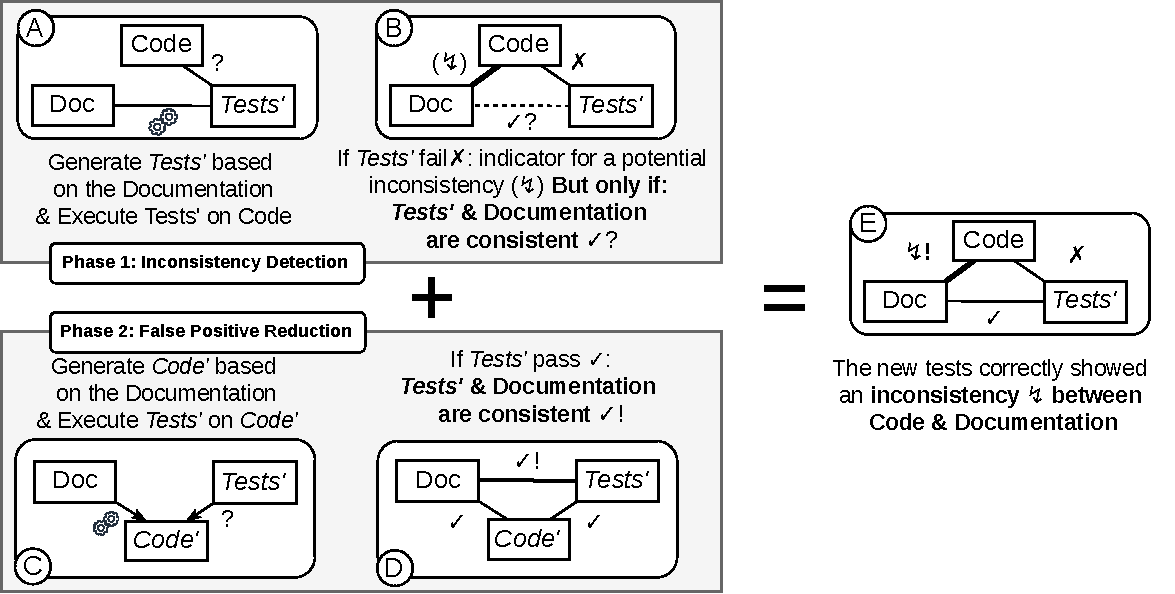
\includegraphics[width=0.8\linewidth]{figures/mainFigure.pdf}
    \caption{Intuition behind CASCADE. Phase 1 detects potential inconsistencies under the assumption that tests and documentation are aligned, and Phase 2 confirms this alignment.}
    \label{fig:idea}
\end{figure}

\subsection{CASCADE's Current Evaluation Metrics}

The original CASCADE paper primarily evaluates the effectiveness of the detection of inconsistencies.
Metrics used here are mainly recall, precision, specificity, pair-wise fix precision (PFP) and F1-score, which are built out of the number of true positives, true negatives, false positives and false negatives.

\begin{equation*}
    rec = \frac{TP}{TP + FN} \quad  prec = \frac{TP}{TP + FP} \quad spec = \frac{TN}{TN + FP} \quad F_1=\frac{2\cdot prec \cdot rec}{prec + rec}
\end{equation*}

\subsection{Quantitative LLM Metrics}

\begin{figure}
    \centering
    \fbox{\parbox{0.85\textwidth}{\centering TODO: Insert architecture or workflow diagram.}}
    \caption{TODO: Baseline workflow or system context.}
    \label{fig:background-workflow}
\end{figure}

\sectioncontributors{Bruno Hemoura}